\chapter{Cognitive Biases}
\markright{Chap \ref{ch:cognitivebiases}: Cognitive Biases}
\label{ch:cognitivebiases}
\setlength{\parindent}{1em}

\section{Introduction}

Humans are complicated. We have limited access to the world around us and yet we've built elaborate tools to let us access even more than we used to imagine could've existed. Each of us comes equipped with a roughly 1.4 kg hunk of fatty tissue we call the `brain' composed of approximately 170 billion cells. Roughly half of these are neurons that compose an elaborate electrical network that reacts to and interacts with the world. This network has evolved over several million years in human beings as we've interacted with and altered the world around us.

Unfortunately, the adaptations that made humans well-suited to their environments during the previous three million years or so aren't necessarily the ones that make us perfect logical reasoners. One reason for this is that perfect logical reasoning is \emph{hard work}. Sometimes it's more cost effective to risk being wrong or making a mistake if the alternative requires you to write out a long, formal argument. Another reason is that sometimes we face problems that can't be solved by detailed logical analysis. If you want your crush to reciprocate your feelings towards them, consider that writing them a lengthy proof may not be the best strategy. If you want to resolve a dispute between two aggreived parties, you may need to do other things before they will listen to a well-reasoned compromise.

Humans are social creatures and so many of the cognitive shortcuts we evolved may be for socially expedient reasons. After all, if you disagree with everyone in your community you are more likely to be made an outcast than to be hailed as a wise seeker of the truth. Socrates was put to death by his fellow Athenians for ``worshipping false gods and corrupting the youth.''

In this chapter we are going to explore some of the cognitive biases that affect us as we try to reason about the world. Many of our cognitive biases are active objects of study by philosophers, cognitive scientists, and psychologists. Before we begin examining these biases in more detail, there are a few things to remark about cognitive biases in general.

First, and perhaps most important, is that \emph{everyone} experiences these biases from time to time. No one is immune to them, because we all get our basic cognitive structure from the same place. Knowing about these biases gives us an advantage as critical thinkers because we can identify and study these biases, but just knowing about them isn't enough to make us better at avoiding them. To get better at that takes practice and conscious effort. Even then, your brain may revert to using a bias without you even realizing it!

Second, just because these patterns of reasoning are biased doesn't necessarily mean that the conclusions drawn from them are always wrong. We can reason in a biased way and still get to the right conclusion. The problem with biases of the sort we're discussing here is that these patterns of reasoning aren't \emph{reliable} at getting us to the truth. They often lead us astray of another conclusion is more expedient. We want to avoid biased reasoning not because it's always wrong but because it is less consistently right.

Third, we are focusing here on cognitive biases, or biases in our reasoning that effect how human beings actually make inferences. There are other kinds of bias---for example, a bias towards preferring certain kinds of food or music---that aren't classified as cognitive in this way. Likewise, there are biases that are distinctly \emph{moral} in character, such as being biased against people who are different from you. These aren't the kinds of biases we have in mind here.

Finally, this isn't an exhaustive or comprehensive list of cognitive biases. Because this area is being actively studied scientists often discover that we are more or less biased than we thought, or that our biases are more sensitive to environmental or social conditions than we first realized. As a good critical thinker, it's worth your time and effort to stay updated on research into human biases and to develop a habit of reflecting on your own reasoning. You may identify biases in your own reasoning that we don't discuss here!

\section{Confirmation Bias}

\textsc{\Gls{confirmation bias}} is the unconscious tendency to discount, ignore, or forget information that contradicts our previously held beliefs. This term was first coined by the psychologist Peter Wason based on his 1960 paper, ``On the failure to eliminate hypotheses in a conceptual task.''\footnote{See \cite{wason1960}.} In the paper Wason conducts the following very elegant experiment. 

He asks participants to perform what is called the ``2-4-6 Task.'' The participants are told that the experimenter has in mind a rule to identify triples of numbers. Every triple either satisfies the rule or doesn't. Participants are then told that the triple $(2,4,6)$ satisfies the rule and they are invited to guess new triples. The experimenter will tell the participants whether or not their guess satisfies the rule.

\textbf{Take a second and think about what the rule Wason used might be. Do you have a guess? What triples would you ask the experimenter for evidence?}

What Wason found was that participants are overwhelmingly likely to guess triples that are \emph{consistent} with their initial guesses about what the rule might be. Most participants guessed extremely specific rules like ``The number in the middle is the average of the other two.'' or ``Three consecutive even numbers.'' These participants would suggest triples like $(5,10,15)$ or $(10,12,14)$, which were confirmed by the experimenter to follow the rule. In fact, the rule is simply ``Any three numbers in ascending order.'' so triples like $(1,7,100)$ or $(-2,0.1,5)$ are also admissible.

The point that Wason drew from his experiment is that participants were more likely to seek evidence that \emph{confirmed} their belief about the rule rather than evidence that would \emph{falsify} or contradict that belief.

How do we fall for confirmation bias in everyday life? One common way is to surround ourselves with sources of evidence---including friends, news sources, or podcasts---that \emph{confirm} our beliefs rather than challenge them. Social media and technology companies use algorithms to provide us with more of what we like. Our horoscope tells us something about ourselves that we already believe, leading us to trust the horoscope.

This might not be so bad if we are looking for movie or restaurant recommendations, but it can have deleterious effects on other aspects of our life. If we are looking for advice for school or our love lives, we might listen to people telling us things we already believe rather than challenging us. Someone who believes they are entitled to something will listen to the person who confirms that belief. Instead, we can fight back against confirmation bias by assessing our sources of evidence impartially, by seeking out multiple sources of evidence, and asking yourself what it would take to change your mind.

This last technique can be especially effective if applied in advance. Consider a person who believes that the Earth is flat. Now suppose this person asked themselves, ``What would it take for me to believe that the Earth is not flat, but is actually round?'' They might decide that \emph{absolutely nothing} could ever convince them otherwise. This is a good sign of bad faith reasoning. Most of our beliefs should be sensitive to \emph{some kind of evidence}, even if that evidence would be hard to obtain. Suppose the flat-Earth believer decides to conduct an experiment for themselves, and they decide if the experimental results go one way they will change their mind and if the results go another way they will stick to their position.

This is the kind of thing that you should do regularly! Consider what sorts of evidence would change your mind. By doing so in advance of collecting evidence you avoid a common fallacy called \textsc{\gls{moving the goalposts}}. This fallacy occurs when some evidence is considered sufficient for some claim $P$, only to deny $P$ once the evidence is provided.

\newglossaryentry{moving the goalposts}
{
name=moving the goalposts,
description={The fallacy of moving the goalposts occurs when someone claims that some piece of evidence would be sufficient for some claim $P$, only to deny that $P$ once the evidence is provided.}
}

\section{Availability Heuristic}

\newglossaryentry{availability heuristic}
{
name=availability heuristic,
description={The availability heuristic occurs when we only attend to the information that is readily available to us.}
}

The \textsc{\gls{availability heuristic}} (also called the ``availability bias'') is closely related to confirmation bias. This bias occurs when we only attend to the information that is readily available to us. Sometimes this is referred to as the ``selective attention bias.'' The idea is that human beings have a limited cognitive capacity and so we're more likely to judge as important the things that we can easily remember or observe, and less likely to judge as important things that are harder to remember or observe.

Psychological work by Kahneman and Tversky showed that people are more likely to remember things that are more ``salient'' in some way.\footnote{\cite{tversky1973}} For example, if ask to memorize a list of names, some of which are ordinary and others are the names of celebrities, participants remember the celebrity names better than the ordinary ones.

Try this. Which do you think is more common: English words that begin with the letter K or English words that have K as the third letter? You probably have an easier time coming up with examples of the former over the latter.

As it turns out, there are roughly three times as many words with K in the third letter position as there are words that begin with K! The explanation for our tendency to think otherwise is that we tend to emphasize the evidence we can recall and deemphasize what we can't. This may be unsurprising, given that we can't treat as evidence something we can't even remember! But it is important to recognize that we may not be seeing all the facts, even if we are trying to collect evidence. Especially when generalizing about something, pay attention to where you are getting your evidence from. Did you make an attempt to collect evidence in an unbiased way?

To avoid falling prey to bad reasoning because of the availability heuristic, try to ask yourself what sources of evidence you may be missing, and to pay special attention to disconfirming evidence.

\section{Anchoring and Ordering Effects}

A psychological consequence of availability is that we often pay attention to only \emph{part} of the available evidence. There are many ways that this can occur; so many so that it would be too large a task to try and list them all.

However, we can categorize many forms of availability bias into \textsc{\gls{anchoring}} and \textsc{\gls{ordering effects}}.

\newglossaryentry{anchoring}
{
name=anchoring,
description={Anchoring occurs when we focus on the initial or most salient information we receive, even when that information is relatively unrepresentative or unhelpful.}
}

Anchoring occurs when we receive some collection of evidence and we use that evidence to establish an unjustified `norm' or \emph{anchor} against which we compare future evidence. A very common form of anchoring is called `price anchoring' and it is well known to advertisers and corporations with an interest in selling you things.

Here's an example of price anchoring. Suppose an ice-cream shop sells three sizes of ice cream: an 6 oz. cup for \$2, a 16 oz cup for \$6, and a 48 oz bucket for \$20. Many people will see the \$20 bucket of ice cream and `anchor' their expectations about the price of the ice cream based on that price. Few people may purchase the \$20 bucket, but more people may be inclined to get the \$6 cup over the \$2 because it's the ``middle choice.''

Consider another example of price anchoring: sale pricing. By telling customers that a \$50 item is now on sale for \$30, the customer will be more likely to believe that the product is \emph{worth} \$50 or that that is the fair price. This may or may not be the case, but more often it makes customers more likely to buy an expensive item if they believe that the true value is even higher. Sometimes, price anchoring can even have the straightforward effect of causing others to believe that a more expensive item is higher quality. This is known as the pricing bias.

Anchoring doesn't only occur in pricing. We also anchor our expectations based on the order that we observe things. \textsc{\Gls{ordering effects}} occur when the order in which we receive information effects our evaluation and recall of that information. For example, if we are given evidence in a sequence and are more likely to recall the first or last pieces of evidence. 

Sometimes the order of information can effect our decisions or evaluations as well. In another study by Kahneman and Tversky, participants were told they would have to quickly calculate a long mathematical equation. Participants were then shown either $1\times 2\times 3\times 4\times 5\times 6\times 7\times 8 = ?$ or  $ 8\times 7\times 6\times 5\times 4\times 3\times 2\times 1 = ?$. 

Because the time that participants were given was so short, they effectively had to reply with an estimate of the answer rather than an explicit calculation. When partipants were shown the former equation (beginning with smaller numbers) the median estimate was $512$; when they were shown the latter equation (beginning with larger numbers), the median estimate was $2,250$. In both cases the participants dramatically underestimated the value, but the underestimation was even worse for participants who began reading the equation with smaller numbers.\footnote{The correct answer is orders of magnitude larger than the median guesses: $40,320$.}

\newglossaryentry{ordering effects}
{
name=ordering effects,
description={Ordering effects occur when the order in which we receive information effects our evaluation and recall of that information. For example, if we are given evidence in a sequence and are more likely to recall the first or last pieces of evidence.}
}

\section{Survivorship Bias}

\newglossaryentry{survivorship bias}
{
name=survivorship bias,
description={A bias towards favoring or focusing on data collected from sources that \emph{survived} some filter or process, rather than being eliminated by it.}
}

During World War II, the U.S. government commissioned many academics to support the war effort. Among them were statisticians at the Statistical Research Group (SRG) at Columbia University, including Abraham Wald. One of the projects that Wald contributed to was identifying how to protect bombers from being shot down.

Consider the plane depicted in figure~\ref{fig:survivorplane}. Military officials at the Center for Naval Analyses had identified the areas where bombers tended to exhibit damage (marked as red dots in the diagram) and were designing ways to add armor to those areas that exhibited the most damage (the wings, center of the fuselage, and the tail). It was thought that by armoring the areas of the planes that showed the most damage the planes would be more likely to survive enemy attacks.

\begin{figure}[!ht]
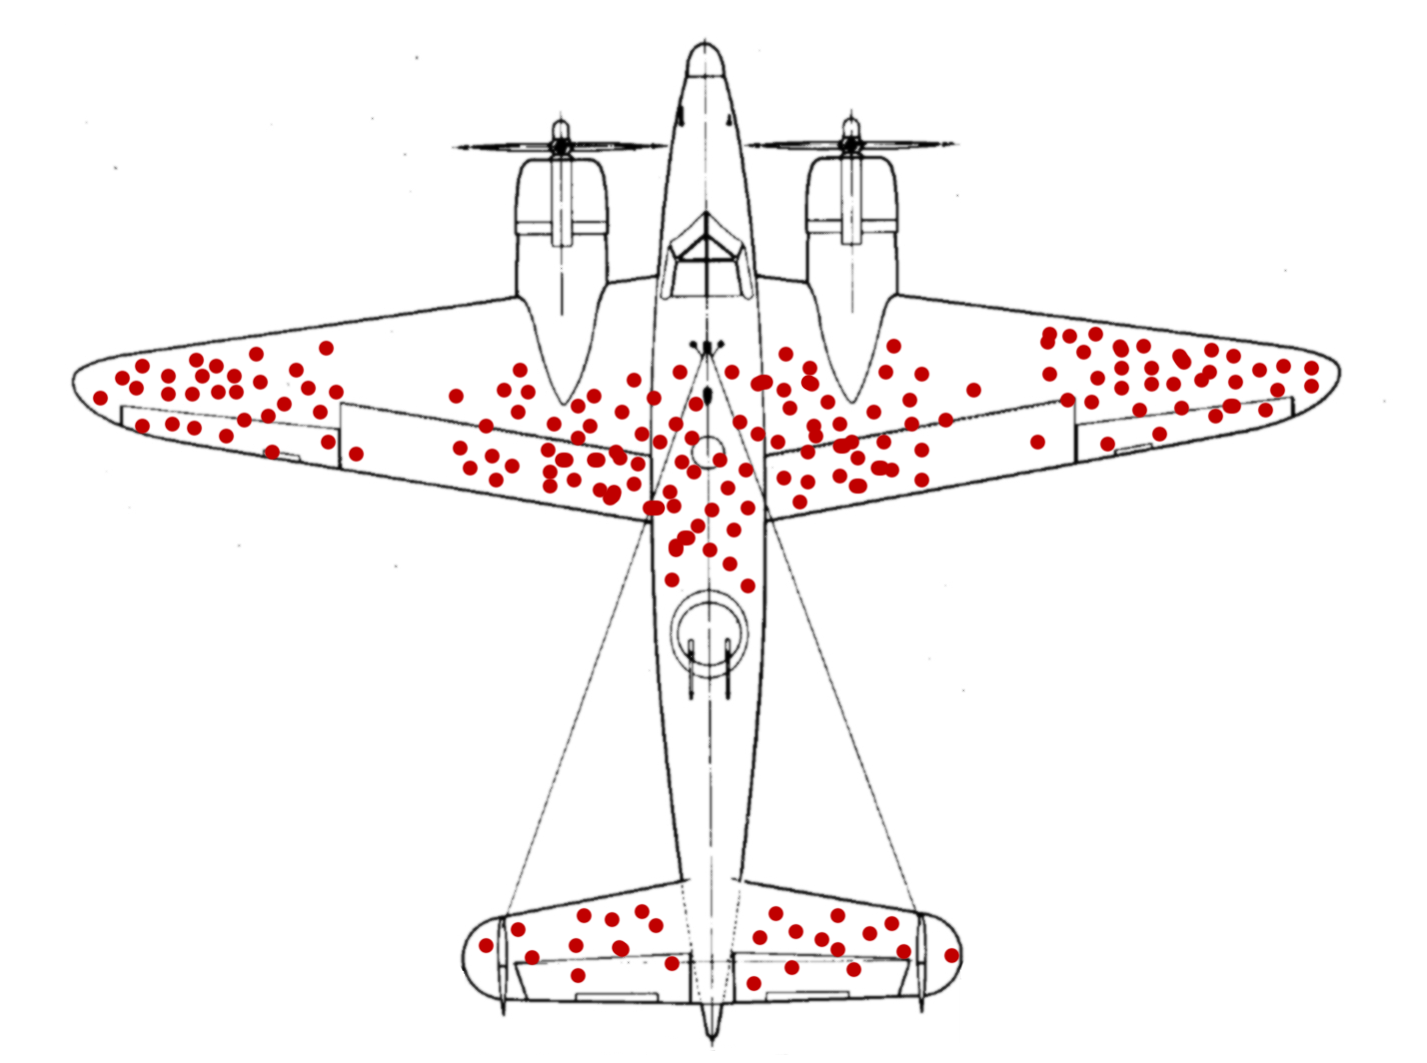
\includegraphics[width=\textwidth]{survivorship-bias}
\caption{A diagram of the locations where damage was recorded on bombers during WWII. Source: \url{https://commons.wikimedia.org/wiki/File:Survivorship-bias.png}}
\label{fig:survivorplane}
\end{figure} 

Wald observed in response to this plan that the data was only collected from the bombers that had \emph{safely returned} from their bombing runs. That is, the damage these planes exhibited was damage that the planes could withstand and still return home. Instead, the military should armor the \emph{undamaged} parts of the plane. This resulted in far fewer planes being shot down and more pilots able to return home.

This is an example of the \textsc{\gls{survivorship bias}}, or a bias towards favoring or focusing on data collected from sources that \emph{survived} some filter or process, rather than being eliminated by it. Prominent examples of survivorship bias include the following:

\begin{enumerate}
\item The belief that the only abortions that occur are the ones reported in hospital records (many abortions occur at home in unsafe conditions due to poverty and lack of healthcare).
\item The belief that music, television, or other media used to be better (there used to be lots of terrible media too, but we don't listen to it any more).
\item The belief that successful CEOs or entrepreneurs have some special ability or talent that enables them to succeed (there are many people who fail due to pure randomness or lack of resources and successful people often start out with many more advantages).
\end{enumerate}

Can you think of other examples of conclusions drawn from evidence biased in this way?

\section{Fundamental Attribution Error}

\newglossaryentry{fundamental attribution error}
{
name=fundamental attribution error,
description={The phenomenon of explaining our own behavior mostly in terms of \emph{external} influences while explaining the behavior of \emph{others} in terms of internal characteristics.}
}

We don't have direct access to anyone's intentions except our own. When we act, we know (more or less) \emph{why} we acted and what we had hoped to achieve by acting. Compare that to how much we know about why other people act. Most of the time we have very little access to anyone else's intentions. We can't hear their thoughts. Sometimes people tell us what they want to achieve, other times we make inferences about what we think their intentions were. This is a difficult task and unsurprisingly we are biased in various ways when we try to achieve it.

The \textsc{\gls{fundamental attribution error}} is the phenomenon of explaining our own behavior mostly in terms of \emph{external} influences like our environment, our circumstances, an illness or a new stressor, etc. while explaining the behavior of \emph{others} in terms of internal characteristics like their character, beliefs, or desires.

As George Carlin once remarked, ``Have you ever noticed that anybody driving slower than you is an idiot, and anyone going faster than you is a maniac?'' The fundamental attribution error causes us to explain away our own behavior and blame others for theirs.

\section{Emotive Biases}

Many philosophers once believed that our emotions and our faculty of reason were in direct competition. They thought that rationality was somehow impeded or stymied by the emotions and that it would be better if we could remain dispassionate, unemotional, and detached. We now know better. Reason and emotion are woven together in a complicated and largely beneficial way. We can measure the ways in which emotion and reason interact both positively and negatively and identify circumstances where emotion can be biasing or completely neutral.

In general, emotive biases are a kind of \textsc{\gls{affect bias}} in which some subject, image, or sensation elicits an emotional response. For example, a strong positive emotional response can sometimes be associated with increased risk taking.\footnote{See e.g. Isen and Patrick (1983) and Anderson and Galinsky (2006).} Here are a few other examples of affect biases:

\textbf{Negativity Bias}: A negativity bias occurs when we attach more evidential significance to negative experiences than to positive ones. This is often manifest in  a belief that negative information is more likely to be true than positive information. Consider political advertisements that attack an opposing candidate, rather than ads that promote the benefits of a candidate's policies.

\textbf{Euphemism/Dysphemism}: Euphemisms and dysphemisms are alternative terms for concepts that are either generally thought of as bad or good, respectively. In other words, these terms are used to shift the \emph{connotation} of a term to have a different value and to elicit a different emotional reaction. An example of a euphemism would be to substitute the term ``freedom fighter'' in place of the term ``terrorist.'' ``Terrorist'' has a generally negative emotional connotation, while the term ``freedom fighter'' seems more positive. 

A dysphemism has a similar effect but in the reverse direction. A dysphemism takes a word or phrase with a generally positive or neutral connotation and replaces it with one that connotes something more negative. The intent is often to communicate that something or someone is bad or immoral by using a more grotesque or dehumanizing term for that person or thing. Slurs and insults can be dysphemisms and dysphemisms can also vary cross-culturally or in different conversational contexts.

Since different concepts elicit different emotional responses in people, what counts as a euphemism or dysphemism is not typically universal. However, it is important to recognize the conversational context one is in or the effects that certain types of communication can have. Context matters, and what once counted as a euphemism may eventually take on the negative affect of the concept it was applied to. Pay attention to the affective response that words have on others to avoid biasing your arguments.

\section{Zeigarnik Effect}

Bluma Zeigarnik was a Soviet psychologist who, among other things, studied memory. After observing that waiters in a cafe were better at remembering the contents of someone's order before they had paid, but after paying the waiter essentially forgot the entire order, Zeigarnik designed several experiments to test this phenomenon.\footnote{\cite{zeigarnik1927}} The effect she found has come to be known as the \textsc{\Gls{Zeigarnik effect}}

\newglossaryentry{Zeigarnik effect}
{
name=Zeigarnik effect,
description={A memory bias according to which people remember the content of uncompleted tasks better than completed tasks.}
}

What she found was that people tend to remember things more accurately and readily if they were interrupted in the middle of their task when compared to cases where they were allowed to complete the task. The proposed explanation is that our brain discards memories that are no longer relevant to us once the task is complete, but uncompleted tasks continue to impose a cognitive load.